\documentclass[11pt]{article}
\title{\textbf{Real data collection}\\
				\large Project for the Internet of Things course @PoliMi Como}
\author{Emanuele Dalla Longa}
\date{2017/11/06}

\usepackage{graphicx}
\usepackage{listings}
\usepackage{amsmath}
\usepackage{hyperref}
\graphicspath{{images/}}
\begin{document}

\maketitle

\section{Introduction}
The aim of this project was to program a TelosB hardware to collect temperature and humidity data from the environment, and broadcast them over the internet, using Node-Red, and analyze them and send the stats via mail. All the code used is available in \href{https://github.com/infinitesnow/IOT2016}{this repository} on GitHub.

\section{Chosen architecture}
I decided to use my Raspberry Pi as a gateway. TelosB was connected over the USB port, and configured to broadcast its output over the serial port. \texttt{node-red} was configured to publish to two online services: Thingspeak (shown in Figure \ref{fig:thingspeak}) and PubNub. From the PubNub channel, I created a Freeboard dashboard to visualize the broadcasted data, as seen in Figure \ref{fig:freeboard}. \texttt{node-red} was configured to send me and a family member a daily report with minimum, maximum and average for each acquired signal for the previous day. All data have been logged into CSV files, which allowed me to plot the data using \texttt{matplotlib}.

\begin{figure}
%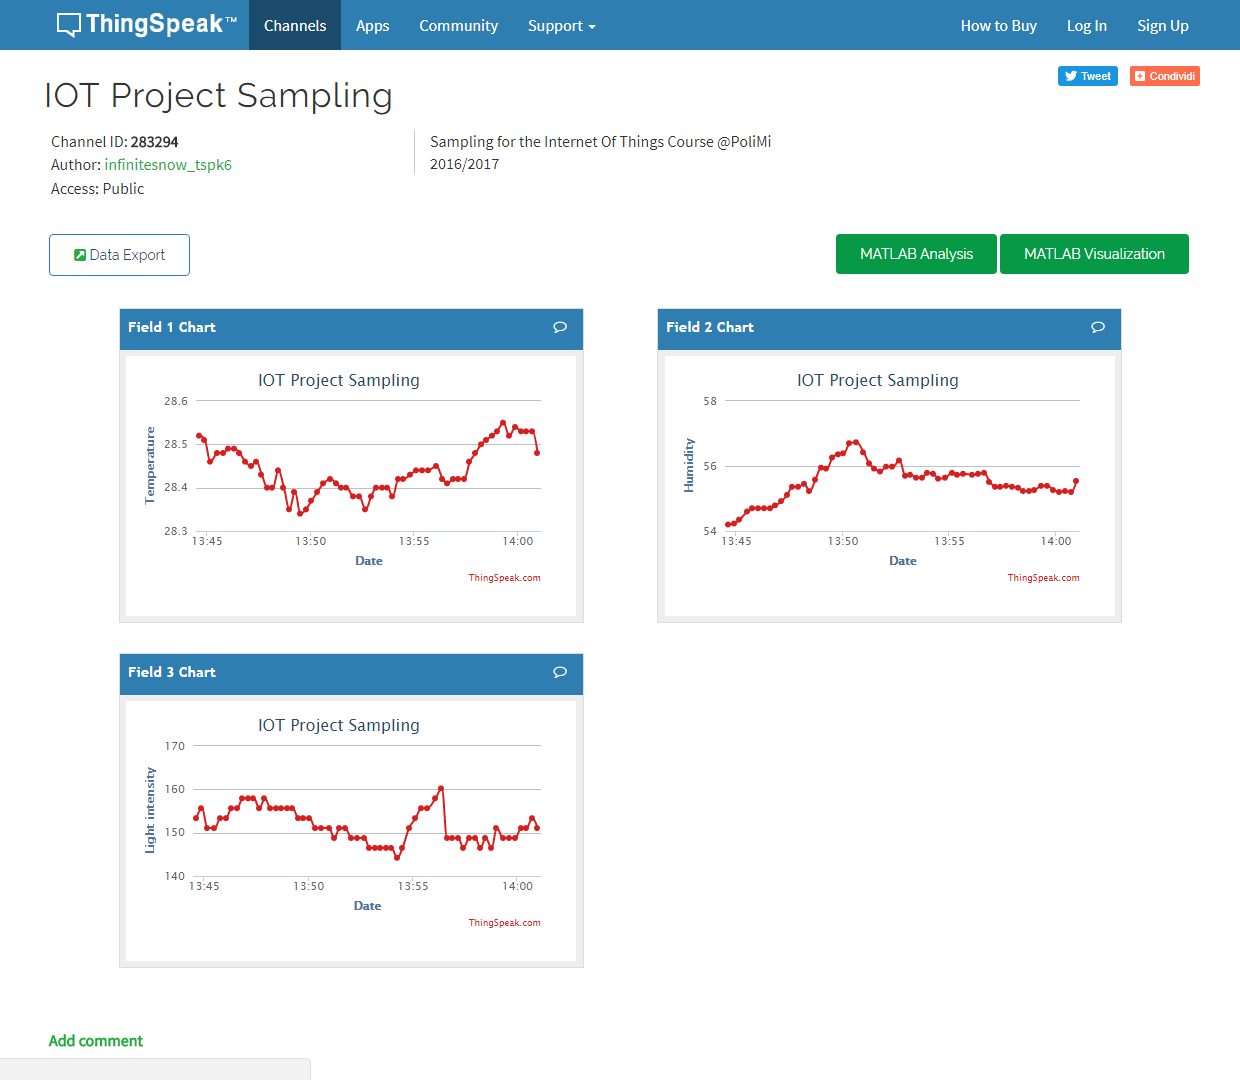
\includegraphics[width=\textwidth]{thingspeak}
\caption{Thingspeak channel}
\label{fig:thingspeak}
\end{figure}

\begin{figure}
%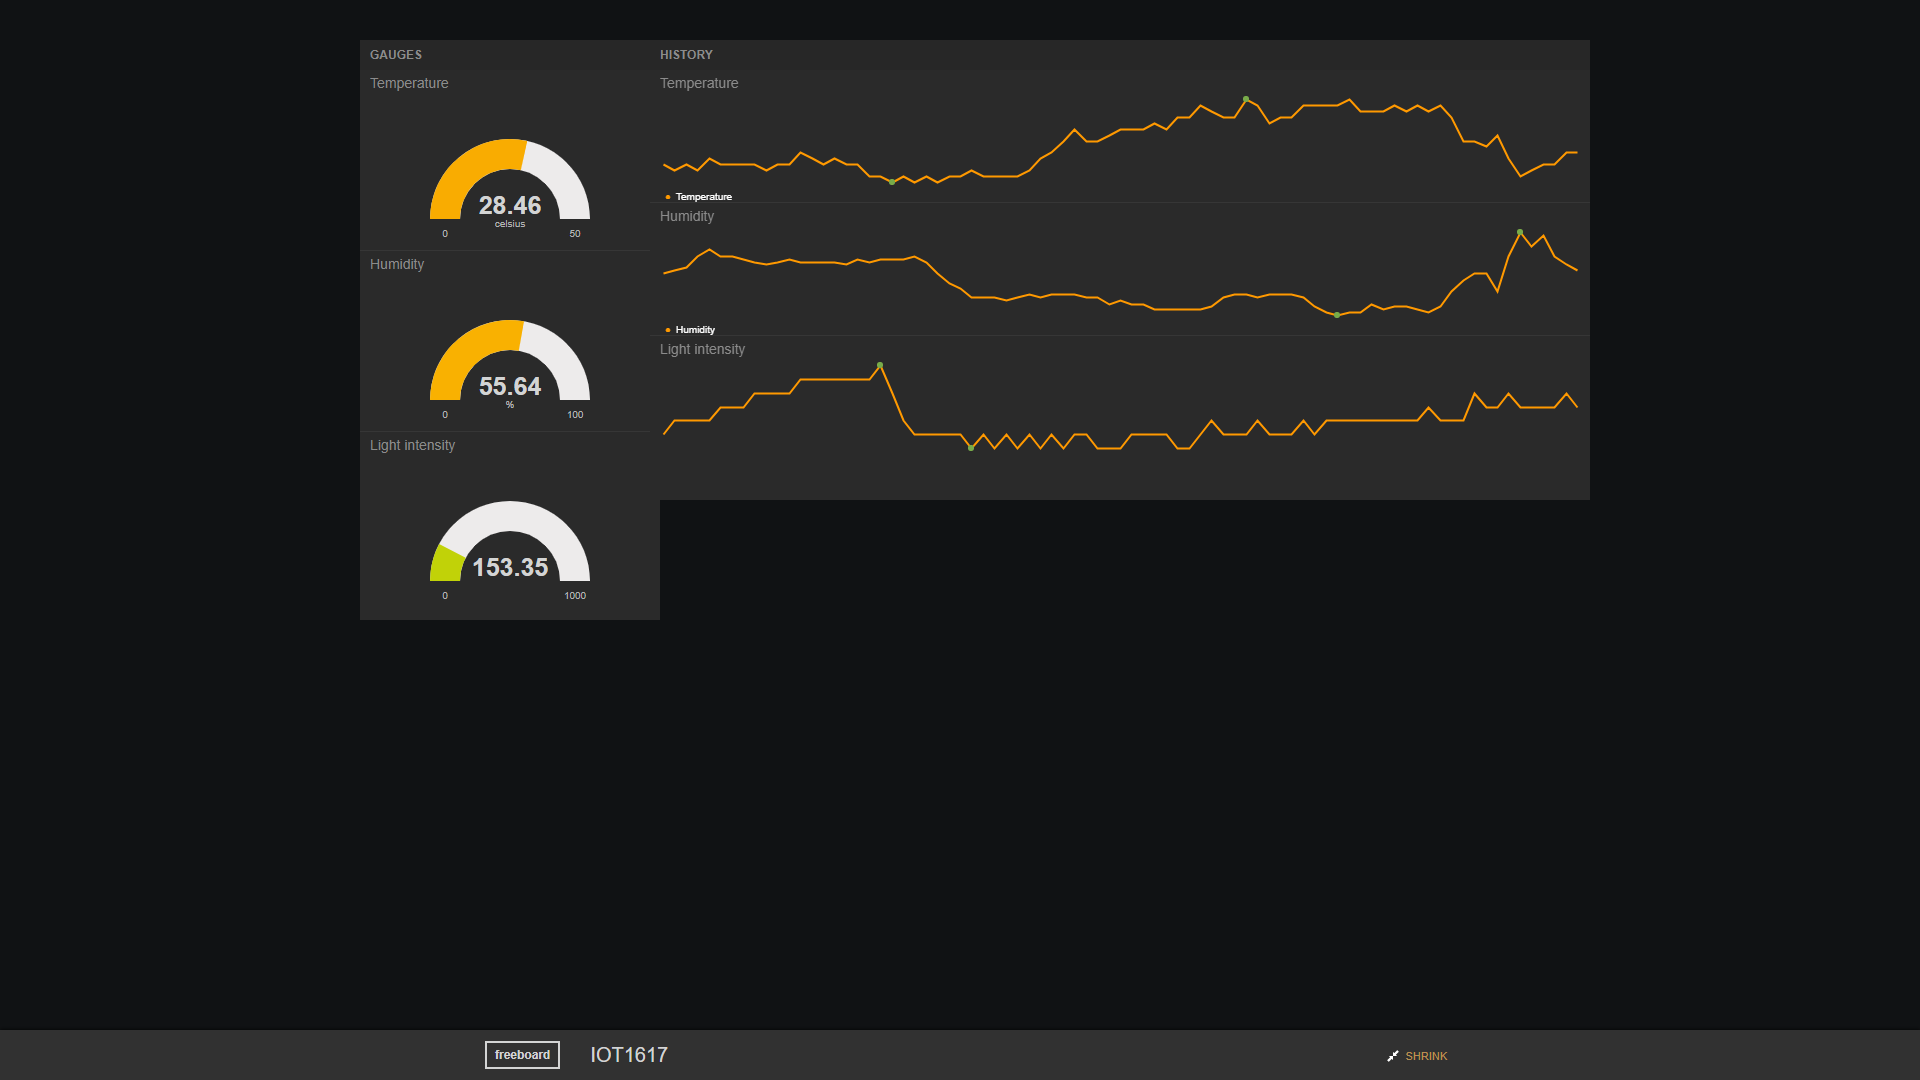
\includegraphics[width=\textwidth]{freeboard}
\caption{Freeboard.io dashboard}
\label{fig:freeboard}
\end{figure}

\section{Reading the serial port}
To read from the serial port, I tried to manually create a script using Python's \texttt{Serial} module, which read chunks of 21 bytes from the input. This worked, but it caused unexpected readings. Splitting on the \texttt{0x7E} flag byte, which is what the TinyOS library provided in \texttt{tinyos.py} file does, seemed to solve the problem. I switched to \texttt{node-red-node-serialport}, which makes this easy to do and integrates cleanly with \texttt{node-red}. But I still had problems, because when a reading had, usually in its least significant byte, the value of the flag byte, the packet got prematurely truncated and the readings went off scale. So, I modified the Python script adding checks on the packet header and footer to ensure correct aligning, and fixed the packet length.  
 
The relevant part of our payload are three \texttt{uint16} sensor readings. Here is the relevant part of the parsing done with Python's \texttt{Serial} module.

\begin{lstlisting}
data_array=struct.unpack_from('>BBBHHBBBHHHHB',data_raw)
\end{lstlisting}

The first byte (\texttt{B}) is always a \texttt{\~} (\texttt{0x7E}), like the last one, and two other \texttt{byte}s. Then we have the header, with two \texttt{unsigned int} for the destination and source address and three \texttt{byte}s for the message length, group ID, and Active Message handler type. The next three \texttt{unsigned int} are our payload, followed by an \texttt{unsigned int} for the footer and a terminator \texttt{byte}.

\section{Sensor calibration}
The sensors I needed to use were a Sensirion SHT11, which provides humidity and temperature readings, and a Humamatsu S1870, which provides visible light intensity. 

I got the transfer function coefficients for the Sensirion sensor from the vendor's datasheet. For the humidity, we have:
$$\text{humidity}=c_1+c_2\cdot x +c_3\cdot x^2$$
where
$$c_1= -2.0468$$
$$c_2=  0.0367$$
$$c_3= -1.5955\cdot10^{-6}$$
for the temperature, we have
$$\text{temperature}=d_1+d_2\cdot x$$ 
$$d_1= -40$$
$$d_2=  0.01$$

On the other hand, I got the Humamatsu conversion factors from the TinyOS wiki. The internal voltage sensor uses the microcontroller's 12-bit ADC: we convert the raw value of the ADC to the corresponding voltage like this:

$$ V_{sensor}=\frac{V_{raw}}{4096} * V_{ref} $$ 

Then, we need the current created by the photodiode through a 100kOhm resistor:

$$I = \frac{ V_{sensor} }{10^5}$$

Finally, the value in lux is calculated using the vendor's datasheet: 

$$\text{light intensity} = 0.625\cdot10^6 \cdot I \cdot 1000$$
  

\section{Sensor data}

We are now going to plot some data acquired from the TelosB board.

\begin{figure}[h]
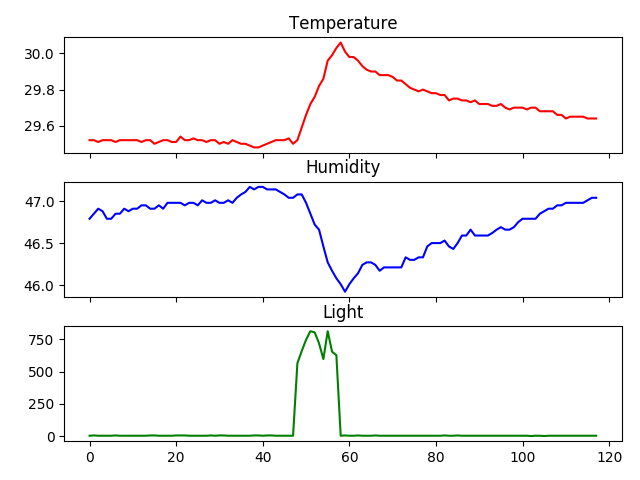
\includegraphics[width=\textwidth]{lamp}
\caption{This is a test plot done on the evening of June 13th. We can see the effect of turning a light bulb lamp on, shedding light directly on the sensor. We see light intensity peaking, temperature rising and humidity dropping.}
\end{figure}

\end{document}
